\section{syscall.h File Reference}
\label{syscall_8h}\index{syscall.h@{syscall.h}}
{\tt \#include $<$sys/types.h$>$}\par
{\tt \#include $<$sys/time.h$>$}\par
{\tt \#include \char`\"{}host.h\char`\"{}}\par
{\tt \#include \char`\"{}misc.h\char`\"{}}\par
{\tt \#include \char`\"{}machine.h\char`\"{}}\par
{\tt \#include \char`\"{}thread.h\char`\"{}}\par


Include dependency graph for syscall.h:\nopagebreak
\begin{figure}[H]
\begin{center}
\leavevmode
\includegraphics[width=420pt]{syscall_8h__incl}
\end{center}
\end{figure}


This graph shows which files directly or indirectly include this file:\nopagebreak
\begin{figure}[H]
\begin{center}
\leavevmode
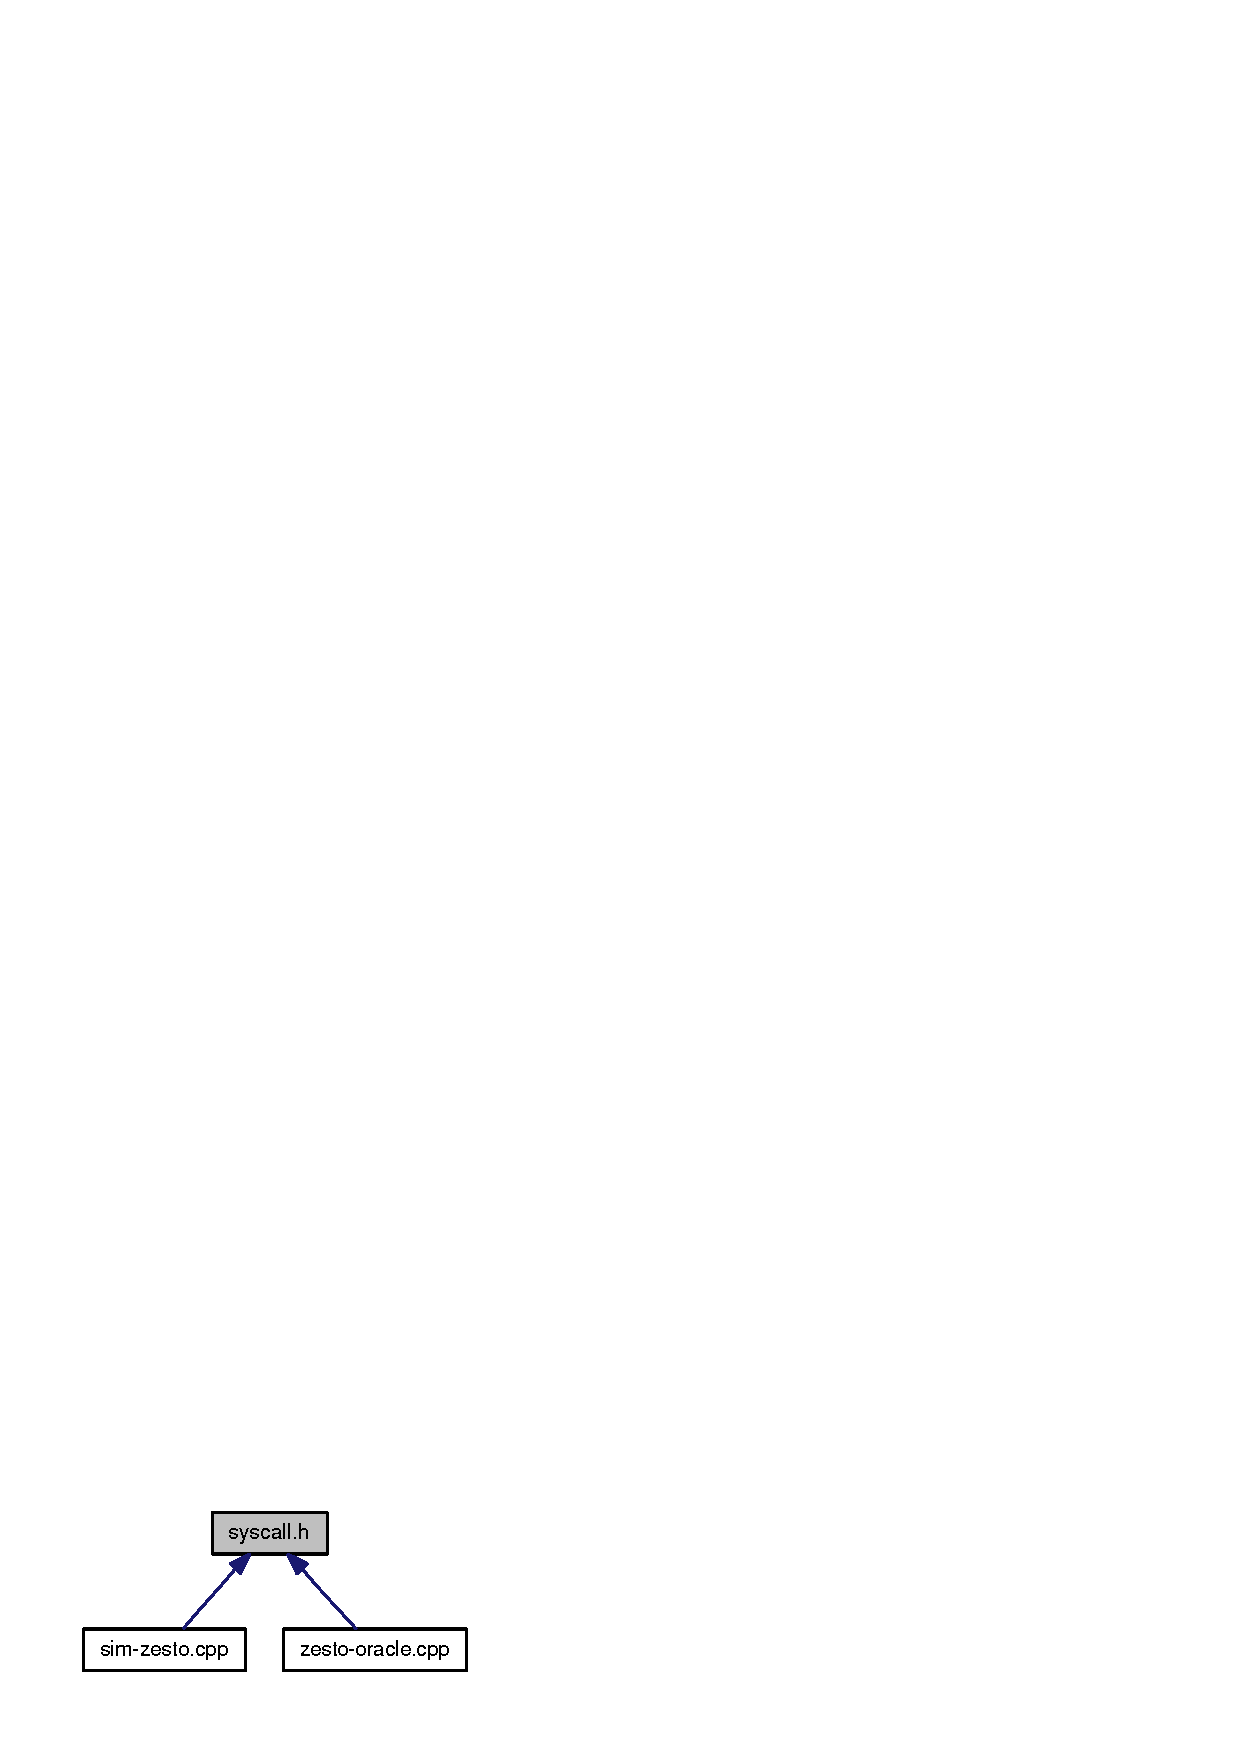
\includegraphics[width=114pt]{syscall_8h__dep__incl}
\end{center}
\end{figure}
\subsection*{Functions}
\begin{CompactItemize}
\item 
void {\bf sys\_\-syscall} (struct {\bf thread\_\-t} $\ast$core, {\bf mem\_\-access\_\-fn} mem\_\-fn, {\bf md\_\-inst\_\-t} inst, int traceable)
\end{CompactItemize}


\subsection{Function Documentation}
\index{syscall.h@{syscall.h}!sys\_\-syscall@{sys\_\-syscall}}
\index{sys\_\-syscall@{sys\_\-syscall}!syscall.h@{syscall.h}}
\subsubsection[{sys\_\-syscall}]{\setlength{\rightskip}{0pt plus 5cm}void sys\_\-syscall (struct {\bf thread\_\-t} $\ast$ {\em core}, \/  {\bf mem\_\-access\_\-fn} {\em mem\_\-fn}, \/  {\bf md\_\-inst\_\-t} {\em inst}, \/  int {\em traceable})}\label{syscall_8h_7b7d5eb9355bf9e9a876e25df407ca6b}


